%% bare_conf_compsoc.tex
%% V1.4b
%% 2015/08/26
%% by Michael Shell
%% See:
%% http://www.michaelshell.org/
%% for current contact information.
%%
%% This is a skeleton file demonstrating the use of IEEEtran.cls
%% (requires IEEEtran.cls version 1.8b or later) with an IEEE Computer
%% Society conference paper.
%%
%% Support sites:
%% http://www.michaelshell.org/tex/ieeetran/
%% http://www.ctan.org/pkg/ieeetran
%% and
%% http://www.ieee.org/

%%*************************************************************************
%% Legal Notice:
%% This code is offered as-is without any warranty either expressed or
%% implied; without even the implied warranty of MERCHANTABILITY or
%% FITNESS FOR A PARTICULAR PURPOSE! 
%% User assumes all risk.
%% In no event shall the IEEE or any contributor to this code be liable for
%% any damages or losses, including, but not limited to, incidental,
%% consequential, or any other damages, resulting from the use or misuse
%% of any information contained here.
%%
%% All comments are the opinions of their respective authors and are not
%% necessarily endorsed by the IEEE.
%%
%% This work is distributed under the LaTeX Project Public License (LPPL)
%% ( http://www.latex-project.org/ ) version 1.3, and may be freely used,
%% distributed and modified. A copy of the LPPL, version 1.3, is included
%% in the base LaTeX documentation of all distributions of LaTeX released
%% 2003/12/01 or later.
%% Retain all contribution notices and credits.
%% ** Modified files should be clearly indicated as such, including  **
%% ** renaming them and changing author support contact information. **
%%*************************************************************************


% *** Authors should verify (and, if needed, correct) their LaTeX system  ***
% *** with the testflow diagnostic prior to trusting their LaTeX platform ***
% *** with production work. The IEEE's font choices and paper sizes can   ***
% *** trigger bugs that do not appear when using other class files.       ***                          ***
% The testflow support page is at:
% http://www.michaelshell.org/tex/testflow/



\documentclass[conference,compsoc]{IEEEtran}
% Some/most Computer Society conferences require the compsoc mode option,
% but others may want the standard conference format.
%
% If IEEEtran.cls has not been installed into the LaTeX system files,
% manually specify the path to it like:
% \documentclass[conference,compsoc]{../sty/IEEEtran}





% Some very useful LaTeX packages include:
% (uncomment the ones you want to load)


% *** MISC UTILITY PACKAGES ***
%
%\usepackage{ifpdf}
% Heiko Oberdiek's ifpdf.sty is very useful if you need conditional
% compilation based on whether the output is pdf or dvi.
% usage:
% \ifpdf
%   % pdf code
% \else
%   % dvi code
% \fi
% The latest version of ifpdf.sty can be obtained from:
% http://www.ctan.org/pkg/ifpdf
% Also, note that IEEEtran.cls V1.7 and later provides a builtin
% \ifCLASSINFOpdf conditional that works the same way.
% When switching from latex to pdflatex and vice-versa, the compiler may
% have to be run twice to clear warning/error messages.






% *** CITATION PACKAGES ***
%
\ifCLASSOPTIONcompsoc
  % IEEE Computer Society needs nocompress option
  % requires cite.sty v4.0 or later (November 2003)
  \usepackage[nocompress]{cite}
\else
  % normal IEEE
  \usepackage{cite}
\fi
% cite.sty was written by Donald Arseneau
% V1.6 and later of IEEEtran pre-defines the format of the cite.sty package
% \cite{} output to follow that of the IEEE. Loading the cite package will
% result in citation numbers being automatically sorted and properly
% "compressed/ranged". e.g., [1], [9], [2], [7], [5], [6] without using
% cite.sty will become [1], [2], [5]--[7], [9] using cite.sty. cite.sty's
% \cite will automatically add leading space, if needed. Use cite.sty's
% noadjust option (cite.sty V3.8 and later) if you want to turn this off
% such as if a citation ever needs to be enclosed in parenthesis.
% cite.sty is already installed on most LaTeX systems. Be sure and use
% version 5.0 (2009-03-20) and later if using hyperref.sty.
% The latest version can be obtained at:
% http://www.ctan.org/pkg/cite
% The documentation is contained in the cite.sty file itself.
%
% Note that some packages require special options to format as the Computer
% Society requires. In particular, Computer Society  papers do not use
% compressed citation ranges as is done in typical IEEE papers
% (e.g., [1]-[4]). Instead, they list every citation separately in order
% (e.g., [1], [2], [3], [4]). To get the latter we need to load the cite
% package with the nocompress option which is supported by cite.sty v4.0
% and later.





% *** GRAPHICS RELATED PACKAGES ***
%
\ifCLASSINFOpdf
  % \usepackage[pdftex]{graphicx}
  % declare the path(s) where your graphic files are
  % \graphicspath{{../pdf/}{../jpeg/}}
  % and their extensions so you won't have to specify these with
  % every instance of \includegraphics
  % \DeclareGraphicsExtensions{.pdf,.jpeg,.png}
\else
  % or other class option (dvipsone, dvipdf, if not using dvips). graphicx
  % will default to the driver specified in the system graphics.cfg if no
  % driver is specified.
  % \usepackage[dvips]{graphicx}
  % declare the path(s) where your graphic files are
  % \graphicspath{{../eps/}}
  % and their extensions so you won't have to specify these with
  % every instance of \includegraphics
  % \DeclareGraphicsExtensions{.eps}
\fi
% graphicx was written by David Carlisle and Sebastian Rahtz. It is
% required if you want graphics, photos, etc. graphicx.sty is already
% installed on most LaTeX systems. The latest version and documentation
% can be obtained at: 
% http://www.ctan.org/pkg/graphicx
% Another good source of documentation is "Using Imported Graphics in
% LaTeX2e" by Keith Reckdahl which can be found at:
% http://www.ctan.org/pkg/epslatex
%
% latex, and pdflatex in dvi mode, support graphics in encapsulated
% postscript (.eps) format. pdflatex in pdf mode supports graphics
% in .pdf, .jpeg, .png and .mps (metapost) formats. Users should ensure
% that all non-photo figures use a vector format (.eps, .pdf, .mps) and
% not a bitmapped formats (.jpeg, .png). The IEEE frowns on bitmapped formats
% which can result in "jaggedy"/blurry rendering of lines and letters as
% well as large increases in file sizes.
%
% You can find documentation about the pdfTeX application at:
% http://www.tug.org/applications/pdftex





% *** MATH PACKAGES ***
%
%\usepackage{amsmath}
% A popular package from the American Mathematical Society that provides
% many useful and powerful commands for dealing with mathematics.
%
% Note that the amsmath package sets \interdisplaylinepenalty to 10000
% thus preventing page breaks from occurring within multiline equations. Use:
%\interdisplaylinepenalty=2500
% after loading amsmath to restore such page breaks as IEEEtran.cls normally
% does. amsmath.sty is already installed on most LaTeX systems. The latest
% version and documentation can be obtained at:
% http://www.ctan.org/pkg/amsmath





% *** SPECIALIZED LIST PACKAGES ***
%
%\usepackage{algorithmic}
% algorithmic.sty was written by Peter Williams and Rogerio Brito.
% This package provides an algorithmic environment fo describing algorithms.
% You can use the algorithmic environment in-text or within a figure
% environment to provide for a floating algorithm. Do NOT use the algorithm
% floating environment provided by algorithm.sty (by the same authors) or
% algorithm2e.sty (by Christophe Fiorio) as the IEEE does not use dedicated
% algorithm float types and packages that provide these will not provide
% correct IEEE style captions. The latest version and documentation of
% algorithmic.sty can be obtained at:
% http://www.ctan.org/pkg/algorithms
% Also of interest may be the (relatively newer and more customizable)
% algorithmicx.sty package by Szasz Janos:
% http://www.ctan.org/pkg/algorithmicx




% *** ALIGNMENT PACKAGES ***
%
%\usepackage{array}
% Frank Mittelbach's and David Carlisle's array.sty patches and improves
% the standard LaTeX2e array and tabular environments to provide better
% appearance and additional user controls. As the default LaTeX2e table
% generation code is lacking to the point of almost being broken with
% respect to the quality of the end results, all users are strongly
% advised to use an enhanced (at the very least that provided by array.sty)
% set of table tools. array.sty is already installed on most systems. The
% latest version and documentation can be obtained at:
% http://www.ctan.org/pkg/array


% IEEEtran contains the IEEEeqnarray family of commands that can be used to
% generate multiline equations as well as matrices, tables, etc., of high
% quality.




% *** SUBFIGURE PACKAGES ***
%\ifCLASSOPTIONcompsoc
%  \usepackage[caption=false,font=footnotesize,labelfont=sf,textfont=sf]{subfig}
%\else
%  \usepackage[caption=false,font=footnotesize]{subfig}
%\fi
% subfig.sty, written by Steven Douglas Cochran, is the modern replacement
% for subfigure.sty, the latter of which is no longer maintained and is
% incompatible with some LaTeX packages including fixltx2e. However,
% subfig.sty requires and automatically loads Axel Sommerfeldt's caption.sty
% which will override IEEEtran.cls' handling of captions and this will result
% in non-IEEE style figure/table captions. To prevent this problem, be sure
% and invoke subfig.sty's "caption=false" package option (available since
% subfig.sty version 1.3, 2005/06/28) as this is will preserve IEEEtran.cls
% handling of captions.
% Note that the Computer Society format requires a sans serif font rather
% than the serif font used in traditional IEEE formatting and thus the need
% to invoke different subfig.sty package options depending on whether
% compsoc mode has been enabled.
%
% The latest version and documentation of subfig.sty can be obtained at:
% http://www.ctan.org/pkg/subfig




% *** FLOAT PACKAGES ***
%
%\usepackage{fixltx2e}
% fixltx2e, the successor to the earlier fix2col.sty, was written by
% Frank Mittelbach and David Carlisle. This package corrects a few problems
% in the LaTeX2e kernel, the most notable of which is that in current
% LaTeX2e releases, the ordering of single and double column floats is not
% guaranteed to be preserved. Thus, an unpatched LaTeX2e can allow a
% single column figure to be placed prior to an earlier double column
% figure.
% Be aware that LaTeX2e kernels dated 2015 and later have fixltx2e.sty's
% corrections already built into the system in which case a warning will
% be issued if an attempt is made to load fixltx2e.sty as it is no longer
% needed.
% The latest version and documentation can be found at:
% http://www.ctan.org/pkg/fixltx2e


%\usepackage{stfloats}
% stfloats.sty was written by Sigitas Tolusis. This package gives LaTeX2e
% the ability to do double column floats at the bottom of the page as well
% as the top. (e.g., "\begin{figure*}[!b]" is not normally possible in
% LaTeX2e). It also provides a command:
%\fnbelowfloat
% to enable the placement of footnotes below bottom floats (the standard
% LaTeX2e kernel puts them above bottom floats). This is an invasive package
% which rewrites many portions of the LaTeX2e float routines. It may not work
% with other packages that modify the LaTeX2e float routines. The latest
% version and documentation can be obtained at:
% http://www.ctan.org/pkg/stfloats
% Do not use the stfloats baselinefloat ability as the IEEE does not allow
% \baselineskip to stretch. Authors submitting work to the IEEE should note
% that the IEEE rarely uses double column equations and that authors should try
% to avoid such use. Do not be tempted to use the cuted.sty or midfloat.sty
% packages (also by Sigitas Tolusis) as the IEEE does not format its papers in
% such ways.
% Do not attempt to use stfloats with fixltx2e as they are incompatible.
% Instead, use Morten Hogholm'a dblfloatfix which combines the features
% of both fixltx2e and stfloats:
%
% \usepackage{dblfloatfix}
% The latest version can be found at:
% http://www.ctan.org/pkg/dblfloatfix

\usepackage{xcolor}
\usepackage{listings}
\usepackage{tikz}
\usepackage{subcaption}
\usepackage{pgfplots}

\usetikzlibrary{shapes.geometric, arrows.meta, positioning}

\tikzset{
    fish/.style={rectangle, draw=green!#1!black, fill=green!#1!white, thick, minimum size=10mm, label=center:\textbf{F}},
    shark/.style={rectangle, draw=blue!#1!black, fill=blue!#1!white, thick, minimum size=10mm, label=center:\textbf{S}}
}

\definecolor{mGreen}{rgb}{0,0.6,0}
\definecolor{mGray}{rgb}{0.5,0.5,0.5}
\definecolor{mPurple}{rgb}{0.58,0,0.82}
\definecolor{backgroundColour}{rgb}{0.95,0.95,0.92}

\lstdefinestyle{CStyle}{
    backgroundcolor=\color{backgroundColour},   
    commentstyle=\color{mGreen},
    keywordstyle=\color{magenta},
    numberstyle=\tiny\color{mGray},
    stringstyle=\color{mPurple},
    basicstyle=\footnotesize,
    breakatwhitespace=false,         
    breaklines=true,                 
    captionpos=b,                    
    keepspaces=true,                 
    numbers=left,                    
    numbersep=5pt,                  
    showspaces=false,                
    showstringspaces=false,
    showtabs=false,                  
    tabsize=2,
    language=C
}


% *** PDF, URL AND HYPERLINK PACKAGES ***
%
%\usepackage{url}
% url.sty was written by Donald Arseneau. It provides better support for
% handling and breaking URLs. url.sty is already installed on most LaTeX
% systems. The latest version and documentation can be obtained at:
% http://www.ctan.org/pkg/url
% Basically, \url{my_url_here}.




% *** Do not adjust lengths that control margins, column widths, etc. ***
% *** Do not use packages that alter fonts (such as pslatex).         ***
% There should be no need to do such things with IEEEtran.cls V1.6 and later.
% (Unless specifically asked to do so by the journal or conference you plan
% to submit to, of course. )


% correct bad hyphenation here
\hyphenation{op-tical net-works semi-conduc-tor}


\begin{document}
%
% paper title
% Titles are generally capitalized except for words such as a, an, and, as,
% at, but, by, for, in, nor, of, on, or, the, to and up, which are usually
% not capitalized unless they are the first or last word of the title.
% Linebreaks \\ can be used within to get better formatting as desired.
% Do not put math or special symbols in the title.
\title{Parallel Simulation of a Cellular Automata Model for \\ Ecosystem Dynamics in a 'Sharks and Fishes' Environment}


% author names and affiliations
% use a multiple column layout for up to three different
% affiliations
\author{\IEEEauthorblockN{John Henry Mejía}
\IEEEauthorblockA{College of Science and Engineering\\
Texas Christian University\\
Fort Worth, Texas 76109 \\
Email: J.H.Mejia@tcu.edu}
% \and
% \IEEEauthorblockN{Homer Simpson}
% \IEEEauthorblockA{Twentieth Century Fox\\
% Springfield, USA\\
% Email: homer@thesimpsons.com}
% \and
% \IEEEauthorblockN{James Kirk\\ and Montgomery Scott}
% \IEEEauthorblockA{Starfleet Academy\\
% San Francisco, California 96678-2391\\
% Telephone: (800) 555--1212\\
% Fax: (888) 555--1212}
}

% conference papers do not typically use \thanks and this command
% is locked out in conference mode. If really needed, such as for
% the acknowledgment of grants, issue a \IEEEoverridecommandlockouts
% after \documentclass

% for over three affiliations, or if they all won't fit within the width
% of the page (and note that there is less available width in this regard for
% compsoc conferences compared to traditional conferences), use this
% alternative format:
% 
%\author{\IEEEauthorblockN{Michael Shell\IEEEauthorrefmark{1},
%Homer Simpson\IEEEauthorrefmark{2},
%James Kirk\IEEEauthorrefmark{3}, 
%Montgomery Scott\IEEEauthorrefmark{3} and
%Eldon Tyrell\IEEEauthorrefmark{4}}
%\IEEEauthorblockA{\IEEEauthorrefmark{1}School of Electrical and Computer Engineering\\
%Georgia Institute of Technology,
%Atlanta, Georgia 30332--0250\\ Email: see http://www.michaelshell.org/contact.html}
%\IEEEauthorblockA{\IEEEauthorrefmark{2}Twentieth Century Fox, Springfield, USA\\
%Email: homer@thesimpsons.com}
%\IEEEauthorblockA{\IEEEauthorrefmark{3}Starfleet Academy, San Francisco, California 96678-2391\\
%Telephone: (800) 555--1212, Fax: (888) 555--1212}
%\IEEEauthorblockA{\IEEEauthorrefmark{4}Tyrell Inc., 123 Replicant Street, Los Angeles, California 90210--4321}}




% use for special paper notices
% \IEEEspecialpapernotice{(Invited Paper)}




% make the title area
\maketitle

% As a general rule, do not put math, special symbols or citations
% in the abstract
\begin{abstract}
This paper presents a parallelized simulation of the cellular automata model for the dynamic interactions between sharks and fishes in a virtual ocean environment. Utilizing C programming language, MPI, and OpenMP, the model efficiently simulates ecosystem behaviors based on defined rules for movement, breeding, and survival within a three-dimensional array. This simulation aims to explore the complexities of predator-prey relationships and the impact of environmental factors like ocean currents on these interactions.

\end{abstract}

% no keywords




% For peer review papers, you can put extra information on the cover
% page as needed:
% \ifCLASSOPTIONpeerreview
% \begin{center} \bfseries EDICS Category: 3-BBND \end{center}
% \fi
%
% For peerreview papers, this IEEEtran command inserts a page break and
% creates the second title. It will be ignored for other modes.
\IEEEpeerreviewmaketitle



\section{Introduction}
% no \IEEEPARstart
Cellular automata provide a powerful tool for simulating complex systems with relatively simple rules. In ecological modeling, cellular automata can simulate the interactions between different species and their environment. This paper discusses the implementation and results of a parallel simulation of an ocean ecosystem populated by sharks and fishes, each following specific behavioral rules in a discrete three-dimensional space.

\section{Background}
The model is inspired by cellular automata like Conway's Game of Life but introduces more complex rules for movement, breeding, and survival, focusing on two species: sharks and fishes. These rules mimic real-world behaviors and interactions in a simplified form. Previous studies have used similar models to study predator-prey dynamics, but few have incorporated the effects of environmental factors like water currents and fully exploited modern parallel computing technologies. Extending this concept to a three-dimensional model populated with sharks and fishes allows for a detailed exploration of predator-prey dynamics and the impact of environmental factors on these interactions. While previous research has often focused on two-dimensional models and overlooked the role of abiotic factors like currents, this study incorporates these elements to enhance the realism and applicability of the simulation. \bibliography{1}


\section{Model Description}

\subsection{Environment}
The simulation environment is a three-dimensional array where each cell can either be empty, contain a fish, or contain a shark. The boundaries of the array are considered edge cells, which have special rules for movement due to fewer adjacent cells. The grid's boundaries conditions are considered reflective boundaries to mimic the natural barriers in a marine environment, such as coastlines or ocean floors.

\subsection{Entities and Rules}

\subsubsection{Fish}

Fish in the simulation exhibit the following behaviors, governed by simple rules:
\begin{enumerate}
\item \textbf{Movement:} A fish moves to an adjacent empty cell. If multiple options are available, one is chosen randomly to simulate non-deterministic movement.
\item \textbf{Breeding:} Upon reaching a predefined age of maturity, a fish can reproduce. This event occurs when the fish moves; it leaves behind a new fish in the cell it vacated, symbolizing the birth of offspring.
\item \textbf{Lifespan:} Each fish has a defined lifespan, after which it dies and its cell becomes empty. This introduces a natural cycle of life and death within the ecosystem.
\end{enumerate}


\subsubsection{Sharks}
Sharks follow a more complex set of rules due to their predatory nature:
\begin{enumerate}
\item \textbf{Feeding and Movement:} If an adjacent cell contains a fish, the shark moves there, consumes the fish, and the cell becomes occupied by the shark. If multiple fish-occupied cells are adjacent, one is selected randomly.
\item \textbf{Starvation:} If a shark does not eat within a certain number of cycles, it dies of starvation. This mechanism controls the shark population and simulates the energy requirements for survival.
\item \textbf{Breeding:} Similar to fish, sharks breed by leaving behind a new shark in their previous location upon moving, provided they have reached a sufficient age of maturity.
\item \textbf{Natural Death:} Sharks also have a maximum lifespan, after which they die even if they have been successful in feeding.
\end{enumerate}

\begin{figure}[h]
\centering
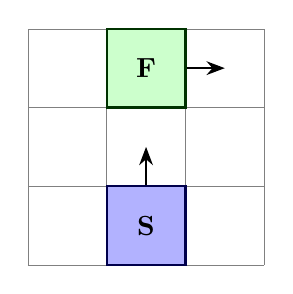
\begin{tikzpicture}
    % Grid setup
    \draw[step=1cm, gray, very thin] (0,0) grid (3,3);
    
    % Fish and Sharks
    \node[draw, fish=20] (fish) at (1.5, 2.5) {};
    \node[draw, shark=30] (shark) at (1.5, 0.5) {};
    
    % Movement arrows
    \draw[-Stealth, thick] (fish) -- (2.5, 2.5);
    \draw[-Stealth, thick] (shark) -- (1.5, 1.5);
\end{tikzpicture}
\caption{Movement of a fish and a shark towards an empty cell.}
\end{figure}

\begin{figure}[h]
    \centering
    
    % Subfigure for the start of the generation
    \begin{subfigure}[b]{0.45\textwidth}
        \centering
        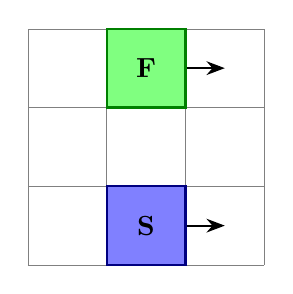
\begin{tikzpicture}
            % Grid setup
            \draw[step=1cm, gray, very thin] (0,0) grid (3,3);
            
            % Fish and Sharks before movement
            \node[draw, circle, fish=50] (fish) at (1.5, 2.5) {};
            \node[draw, circle, shark=50] (shark) at (1.5, 0.5) {};
            
            % Movement arrows
            \draw[-Stealth, thick] (fish) -- (2.5, 2.5);
            \draw[-Stealth, thick] (shark) -- (2.5, 0.5);
        \end{tikzpicture}
        \caption{Start of generation}
    \end{subfigure}
    \hfill % Space between the figures
    % Subfigure for the end of the generation
    \begin{subfigure}[b]{0.45\textwidth}
        \centering
        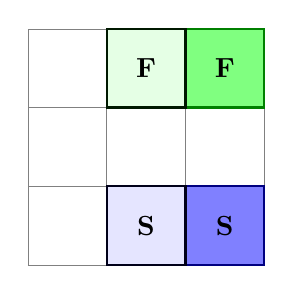
\begin{tikzpicture}
            % Grid setup
            \draw[step=1cm, gray, very thin] (0,0) grid (3,3);
            
            % Fish and Sharks after movement
            \node[draw, circle, fish=50] (fish) at (2.5, 2.5) {};
            \node[draw, circle, shark=50] (shark) at (2.5, 0.5) {};
            
            % Newborns
            \node[draw, circle, fish=10] at (1.5, 2.5) {};
            \node[draw, circle, shark=10] at (1.5, 0.5) {};
            
        \end{tikzpicture}
        \caption{End of generation}
    \end{subfigure}
    
    \caption{Breeding and movement: Both fish and shark leave behind a new offspring in their previous location.}
\end{figure}


\subsection{Currents}

Currents introduce a directional bias to the movement probabilities of both sharks and fishes. Each cycle, the current can shift direction and strength, influencing movement decisions. The strength of the current affects the likelihood of organisms moving in the current's direction, adding a layer of complexity to the simulation by mimicking the dynamic nature of oceanic water movements. Currents can significantly impact the strategies of predator and prey, potentially facilitating escapes or aiding predators in pursuit.

\subsection{Simulation Parameters}
Users can input several parameters at the start of the simulation:
\begin{itemize}
\item \textbf{Size of the ocean:} Defines the dimensions of the three-dimensional grid.
\item \textbf{Initial population:} The number of sharks and fishes and their initial placement.
\item \textbf{Breeding ages:} The age at which sharks and fishes can start breeding.
\item \textbf{Lifespan:} The maximum number of cycles a shark or fish can live.
\item \textbf{Starvation time for sharks:} The number of cycles a shark can go without eating before it starves.
\item \textbf{Current strength and direction:} Initial and variable parameters that influence movement decisions each cycle.
\end{itemize}

This detailed modeling approach, combined with the use of advanced parallel computing techniques, allows for the efficient and realistic simulation of ecological dynamics within a marine environment, providing valuable insights into the balance of ecosystems and the role of environmental factors in shaping biological interactions.



\section{Implementation}

The simulation of the "Sharks and Fishes" model is implemented using a hybrid parallel computing approach that leverages both the Message Passing Interface (MPI) and Open Multi-Processing (OpenMP). This section details the implementation strategy, focusing on parallelization, data structures, and the algorithmic steps involved in each simulation cycle.


\subsection{Parallelization}

The computational challenge of simulating a large ocean ecosystem with numerous entities and interactions is addressed through parallel processing. The parallelization strategy is two-fold:

\begin{enumerate}
\item \textbf{MPI for Distributed Computing:} The ocean grid is partitioned into sub-grids, each managed by a different processor. MPI is used for handling communication between these processors.  Each process should be able to compute the inner part of the assigned block straight away. However computing the new generation values for the 6 sides of each ocean block cannot be done very easily. That is because, the border cells have neighbors residing in another block. Consequently, inter-process communication (i.e: message passing) is required in order for the current process to fetch the values of those neighbors. (See Figure 3)

\item \textbf{OpenMP for Multi-threading:} Within each processor, multiple threads are spawned using OpenMP to handle the computations for each sub-grid. This approach takes advantage of multi-core processors to perform concurrent operations within each sub-grid, such as calculating movements, breeding events, and mortality.
\end{enumerate}

This hybrid model ensures that the simulation can efficiently utilize available hardware resources, minimizing computation time and handling large-scale simulations effectively.

\begin{figure}[!t]
\centering
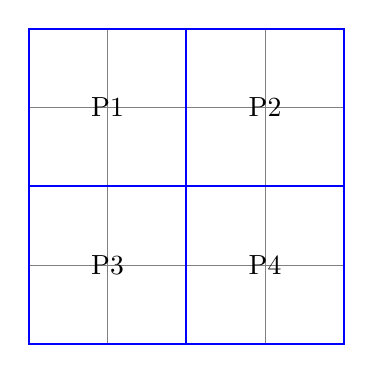
\begin{tikzpicture}
    \draw[step=1cm, gray, very thin] (0,0) grid (4,4);
    \foreach \x in {0,2}
        \foreach \y in {0,2}
            \draw[thick, blue] (\x,\y) rectangle (\x+2,\y+2);
    \node at (1,3) {P1};
    \node at (3,3) {P2};
    \node at (1,1) {P3};
    \node at (3,1) {P4};
\end{tikzpicture}
\caption{Example of how each processor takes their own subsection of the ocean.}
\label{fig_sim}
\end{figure}


% \begin{figure}[!t]
% \centering
% \begin{tikzpicture}
%     \draw[step=1cm, gray, very thin] (0,0) grid (4,4);
%     \draw[fill=blue!50] (1,2) rectangle (2,3); % Shark
%     \draw[fill=green!50] (2,2) rectangle (3,3); % Fish
%     \draw[->, thick] (1.5,2.5) -- (2.5,2.5); % Movement arrow
%     \node at (1.5, 2.5) {\textbf{S}};
%     \node at (2.5, 2.5) {\textbf{F}};
% \end{tikzpicture}
% \caption{Showing Movement Calculation (OpenMP)}
% \label{fig_sim}
% \end{figure}

% \begin{tikzpicture}
%     \draw[step=1cm, gray, very thin] (0,0) grid (4,4);
%     \draw[fill=blue!50] (1,2) rectangle (2,3); % Shark
%     \draw[fill=green!50] (2,2) rectangle (3,3); % Fish
%     \node at (1.5, 2.5) {\textbf{S}};
%     \node at (2.5, 2.5) {\textbf{F}};
%     \draw[fill=green!20] (3,2) rectangle (4,3); % New fish (breeding)
%     \node at (3.5, 2.5) {\textbf{F}};
%     \draw[fill=gray!50] (0,3) rectangle (1,4); % Dead fish
% \end{tikzpicture}

% \begin{tikzpicture}
%     \draw[step=1cm, gray, very thin] (0,0) grid (4,4);
%     \foreach \x in {0,2}
%         \foreach \y in {0,2}
%             \draw[thick, red] (\x,\y) rectangle (\x+2,\y+2);
%     \draw[->, thick, red] (2,2.5) -- (2,3.5); % Communication arrow
%     \draw[->, thick, red] (2,1.5) -- (2,0.5); % Communication arrow
% \end{tikzpicture}

\subsection{Issues with Parallelization}

\subsubsection{Issues Arising from Movement Order}
\begin{itemize}
    \item \textbf{Predation Timing:} If sharks move before fish, they might miss opportunities to eat because fish that would have been in an adjacent cell could have already moved away. Conversely, if fish move first, sharks might have more opportunities to eat because they immediately follow the fish movements.
    \item \textbf{Reproduction and Death:} Reproduction and Death: The timing of movement can affect breeding and death due to age or starvation. For example, if a shark moves and breeds before a neighboring fish that was also due to breed, the new shark might occupy a space that could have been taken by a new fish.
    \item \textbf{Space Occupation:}  Movement order affects how space is occupied. If fish move and fill up spaces first, sharks might find fewer empty cells to move into, affecting their ability to survive if they are on the brink of starvation.
\end{itemize}

\subsubsection{Simulation Steps}
The simulation of the "Sharks and Fishes" model follows a sequential order of operations to ensure clarity and manage the complexity of interactions. Here are the detailed steps:

\begin{enumerate}
    \item \textbf{Sharks Starve or Die:} Update the state of each shark based on its hunger and age. Sharks that haven't eaten within a specified number of generations die of starvation. Sharks also die of natural causes after reaching a certain age.
    \item \textbf{Fish Die:} Update the state of each fish based on their age, with fish dying off after reaching a specified lifespan.
    \item \textbf{Sharks Determine Movement:} Each shark decides whether to move based on the presence of adjacent fish (for feeding) or empty cells (for moving).
    \item \textbf{Fish Determine Movement:} Each fish decides its next move based on the availability of adjacent empty cells.
    \item \textbf{Sharks Move and Eat:} Sharks execute their movements. If a move results in a shark occupying the same cell as a fish, the fish is eaten, and the shark's hunger is reset.
    \item \textbf{Fish Move and Give Birth:} Fish execute their movements. Fish that are old enough to breed leave behind a new fish in their original cell.
    \item \textbf{Shark Breeding:} Sharks that are old enough to breed leave behind a new shark in their original cell.
    \item \textbf{Update Ages and Hunger Levels:} Increment the age of all fish and sharks. For sharks that did not eat this turn, increase their hunger level.
\end{enumerate}

\subsection{Data Structures}

The core data structure is a three-dimensional array of Cells representing the ocean. Each cell in this array can be empty or contain an instance of a `Fish` or `Shark` structure. These structures are defined as follows:

For fish:
\begin{lstlisting}[style=CStyle]
typedef struct {
int age;
int breedAge;
int maxAge;
} Fish;
\end{lstlisting}

For sharks:
\begin{lstlisting}[style=CStyle]
typedef struct {
int age;
int breedAge;
int maxAge;
int starveTime;
int timeSinceLastMeal;
} Shark;
\end{lstlisting}

Each Fish and Shark structure contains fields to track the age, breeding age, and maximum age. Additionally, the Shark structure includes fields to manage its starvation mechanics, crucial for simulating predator dynamics.

\subsection{Algorithm}

Each simulation step involves: 

\begin{enumerate}
\item \textbf{Movement:} 
    \begin{itemize}
        \item Each thread calculates potential moves for sharks and fish within its sub-grid.
        \item Fish move to random adjacent empty cells, while sharks move towards adjacent cells containing fish if available, or randomly otherwise.
        \item Movement decisions are influenced by current strength and direction, which are simulated as bias probabilities affecting the random choice of cells.
    \end{itemize}
\item \textbf{Breeding and Death:}
    \begin{itemize}
        \item After movement, each organism's age is incremented.
        \item Breeding occurs if an organism has moved and meets the age criteria: a new organism of the same type is created in the vacated cell.
        \item Death is checked by age for both species and by starvation for sharks. Cells containing organisms that die are marked empty.
    \end{itemize}
\item \textbf{State update for the Ocean:}
    \begin{itemize}
        \item Once all movements, breeding, and death events are processed, the state of the sub-grid is updated.
        \item This involves writing the new state of each cell back to the main grid structure, ensuring consistency before the next simulation step.
    \end{itemize}
\item \textbf{Inter-processor Communication:}
    \begin{itemize}
        \item After updating local sub-grids, changes at the boundaries of each sub-grid require synchronization with adjacent sub-grids managed by other processors
        \item MPI is used to exchange boundary data among processors to ensure that the next simulation step starts with a consistent global state.
        \item Efficient communication strategies, such as non-blocking sends and receives, are employed to overlap communication with computation, reducing idle times.
    \end{itemize}
\end{enumerate}

\subsection{Performance Considerations}

The performance of the simulation is critically dependent on the efficiency of the parallel algorithms and the effectiveness of the communication strategy. Load balancing, where each processor handles approximately equal amounts of work, is crucial for achieving optimal performance. Dynamic workload adjustments and adaptive sub-grid sizing based on organism density and activity levels are potential enhancements to improve scalability and efficiency.

Currently, sub-grid sizing is based on splitting the grid into levels of the ocean, and providing each grid

This implementation framework sets the foundation for a robust simulation of ecological dynamics in a marine environment, providing insights into complex biological and environmental interactions through high-performance computing techniques.

% An example of a floating figure using the graphicx package.
% Note that \label must occur AFTER (or within) \caption.
% For figures, \caption should occur after the \includegraphics.
% Note that IEEEtran v1.7 and later has special internal code that
% is designed to preserve the operation of \label within \caption
% even when the captionsoff option is in effect. However, because
% of issues like this, it may be the safest practice to put all your
% \label just after \caption rather than within \caption{}.
%
% Reminder: the "draftcls" or "draftclsnofoot", not "draft", class
% option should be used if it is desired that the figures are to be
% displayed while in draft mode.
%
%\begin{figure}[!t]
%\centering
%\includegraphics[width=2.5in]{myfigure}
% where an .eps filename suffix will be assumed under latex, 
% and a .pdf suffix will be assumed for pdflatex; or what has been declared
% via \DeclareGraphicsExtensions.
%\caption{Simulation results for the network.}
%\label{fig_sim}
%\end{figure}

% Note that the IEEE typically puts floats only at the top, even when this
% results in a large percentage of a column being occupied by floats.


% An example of a double column floating figure using two subfigures.
% (The subfig.sty package must be loaded for this to work.)
% The subfigure \label commands are set within each subfloat command,
% and the \label for the overall figure must come after \caption.
% \hfil is used as a separator to get equal spacing.
% Watch out that the combined width of all the subfigures on a 
% line do not exceed the text width or a line break will occur.
%
%\begin{figure*}[!t]
%\centering
%\subfloat[Case I]{\includegraphics[width=2.5in]{box}%
%\label{fig_first_case}}
%\hfil
%\subfloat[Case II]{\includegraphics[width=2.5in]{box}%
%\label{fig_second_case}}
%\caption{Simulation results for the network.}
%\label{fig_sim}
%\end{figure*}
%
% Note that often IEEE papers with subfigures do not employ subfigure
% captions (using the optional argument to \subfloat[]), but instead will
% reference/describe all of them (a), (b), etc., within the main caption.
% Be aware that for subfig.sty to generate the (a), (b), etc., subfigure
% labels, the optional argument to \subfloat must be present. If a
% subcaption is not desired, just leave its contents blank,
% e.g., \subfloat[].


% An example of a floating table. Note that, for IEEE style tables, the
% \caption command should come BEFORE the table and, given that table
% captions serve much like titles, are usually capitalized except for words
% such as a, an, and, as, at, but, by, for, in, nor, of, on, or, the, to
% and up, which are usually not capitalized unless they are the first or
% last word of the caption. Table text will default to \footnotesize as
% the IEEE normally uses this smaller font for tables.
% The \label must come after \caption as always.
%
%\begin{table}[!t]
%% increase table row spacing, adjust to taste
%\renewcommand{\arraystretch}{1.3}
% if using array.sty, it might be a good idea to tweak the value of
% \extrarowheight as needed to properly center the text within the cells
%\caption{An Example of a Table}
%\label{table_example}
%\centering
%% Some packages, such as MDW tools, offer better commands for making tables
%% than the plain LaTeX2e tabular which is used here.
%\begin{tabular}{|c||c|}
%\hline
%One & Two\\
%\hline
%Three & Four\\
%\hline
%\end{tabular}
%\end{table}


% Note that the IEEE does not put floats in the very first column
% - or typically anywhere on the first page for that matter. Also,
% in-text middle ("here") positioning is typically not used, but it
% is allowed and encouraged for Computer Society conferences (but
% not Computer Society journals). Most IEEE journals/conferences use
% top floats exclusively. 
% Note that, LaTeX2e, unlike IEEE journals/conferences, places
% footnotes above bottom floats. This can be corrected via the
% \fnbelowfloat command of the stfloats package.


\section{Performance Analysis}

\subsection{Setup}
The performance analysis of the 3D Sharks and Fish simulation was conducted on a distributed computing environment consisting of multiple nodes, each equipped with a multi-core processor. The simulation was implemented using MPI for inter-node communication and OpenMP for intra-node parallelism. The following parameters were varied during the tests:
\begin{itemize}
    \item Number of processes (MPI ranks): ranging from 4 to 64, doubling at each step.
    \item Number of threads per process: fixed at 4, 8, and 16 threads in different test runs.
    \item Grid size: tested with $100 \times 100 \times 100$, $200 \times 200 \times 200$, and $300 \times 300 \times 300$ cells.
    \item Simulation duration: 1000 generations.
\end{itemize}

\subsection{Results}
The results are presented in two parts: execution time and computational load distribution. Execution time was measured from the start to the end of the simulation, including initialization and data communication between processes.


\begin{figure}
    \centering
    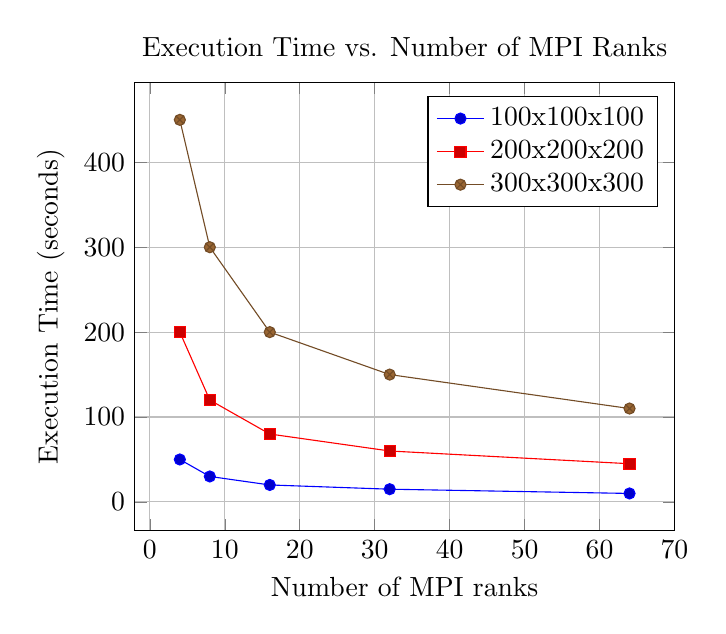
\begin{tikzpicture}
        \begin{axis}[
            xlabel={Number of MPI ranks},
            ylabel={Execution Time (seconds)},
            legend pos=north east,
            title={Execution Time vs. Number of MPI Ranks},
            grid=major]
        \addplot coordinates {(4,50) (8,30) (16,20) (32,15) (64,10)};
        \addlegendentry{100x100x100}
        \addplot coordinates {(4,200) (8,120) (16,80) (32,60) (64,45)};
        \addlegendentry{200x200x200}
        \addplot coordinates {(4,450) (8,300) (16,200) (32,150) (64,110)};
        \addlegendentry{300x300x300}
        \end{axis}
    \end{tikzpicture}
    \caption{Execution time for different grid sizes as a function of the number of MPI ranks.}
    \label{fig:exec_time}
\end{figure}

\subsection{Scalability}
Scalability was assessed by analyzing how the execution time decreases as the number of MPI ranks and threads increases. The simulation shows good scalability up to 32 MPI ranks but begins to level off beyond this point, especially for larger grid sizes. This behavior suggests that communication overhead becomes significant as the number of processes increases.

\subsubsection{Thread Scalability Analysis}

This subsection analyzes the impact of varying the number of OpenMP threads per MPI process on the performance of the simulation. The grid size was fixed at $200 \times 200 \times 200$ for these tests, and the number of MPI ranks was fixed at 16 and 32 to observe the effects under different levels of parallelism.

\begin{figure}[htbp]
    \centering
    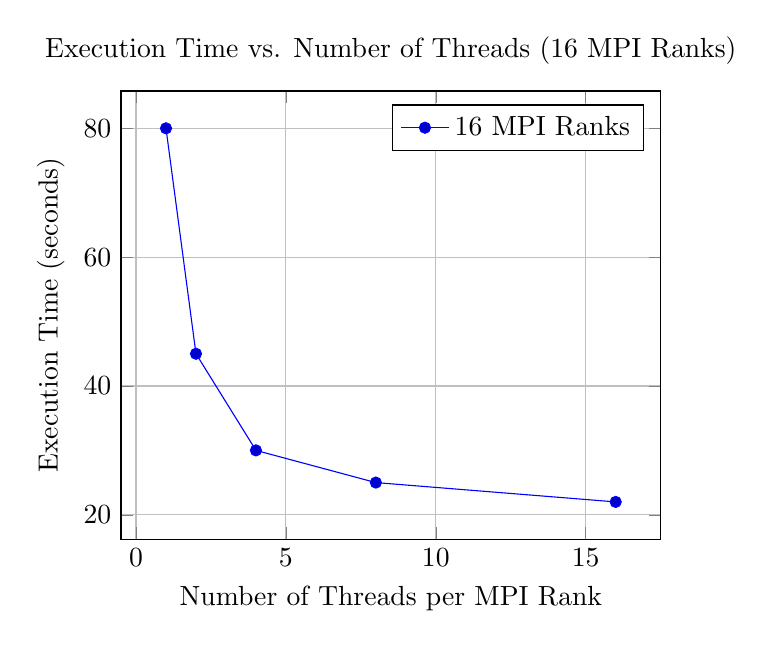
\begin{tikzpicture}
        \begin{axis}[
            xlabel={Number of Threads per MPI Rank},
            ylabel={Execution Time (seconds)},
            legend pos=north east,
            title={Execution Time vs. Number of Threads (16 MPI Ranks)},
            grid=major]
        \addplot coordinates {(1, 80) (2, 45) (4, 30) (8, 25) (16, 22)};
        \addlegendentry{16 MPI Ranks}
        \end{axis}
    \end{tikzpicture}
    \caption{Execution time as a function of the number of OpenMP threads per MPI rank for a fixed grid size of $200 \times 200 \times 200$ cells with 16 MPI ranks.}
    \label{fig:threads_16}
\end{figure}

\begin{figure}[htbp]
    \centering
    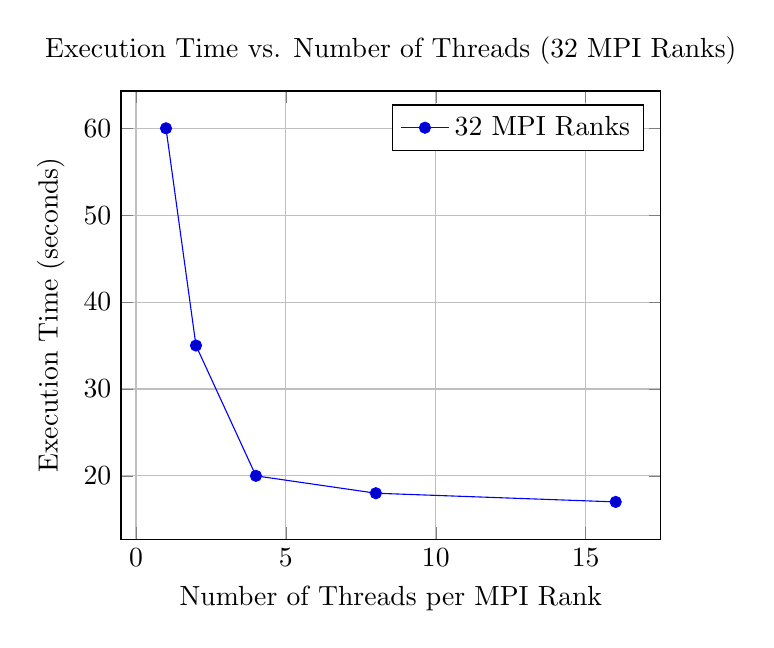
\begin{tikzpicture}
        \begin{axis}[
            xlabel={Number of Threads per MPI Rank},
            ylabel={Execution Time (seconds)},
            legend pos=north east,
            title={Execution Time vs. Number of Threads (32 MPI Ranks)},
            grid=major]
        \addplot coordinates {(1, 60) (2, 35) (4, 20) (8, 18) (16, 17)};
        \addlegendentry{32 MPI Ranks}
        \end{axis}
    \end{tikzpicture}
    \caption{Execution time as a function of the number of OpenMP threads per MPI rank for a fixed grid size of $200 \times 200 \times 200$ cells with 32 MPI ranks.}
    \label{fig:threads_32}
\end{figure}

The results show a clear trend of decreasing execution time as the number of threads increases, up to a certain point. With 16 MPI ranks, the improvement in execution time begins to plateau at 8 threads, suggesting that further increases in thread count provide diminishing returns. A similar pattern is observed with 32 MPI ranks, although the plateau appears at a slightly higher thread count, likely due to the reduced workload per rank.

This behavior underscores the importance of choosing an appropriate number of threads based on the specific hardware and workload characteristics. It also highlights the potential for thread-level contention or resource saturation, which can limit the benefits of increased parallelism at higher thread counts.

\section{Discussion}
The scalability limitation observed in the simulation can be attributed primarily to the increased communication overhead among MPI processes in a 3D grid setup. As the number of processes increases, the fraction of boundary cells requiring inter-process communication grows, impacting overall performance. Additionally, the fixed number of threads per process suggests that there might be an optimal thread count beyond which no significant performance gains can be observed, possibly due to resource contention on the nodes.



\section{Conclusion}
The 3D Sharks and Fish simulation demonstrates effective use of MPI and OpenMP to model complex ecological interactions in a distributed computing environment. While the simulation scales well up to a certain number of processes, further scalability is hindered by inter-process communication overhead. The results provide valuable insights into the trade-offs between computation and communication in large-scale simulations.

\section{Future Work}
Future enhancements to the simulation could focus on several areas:
\begin{itemize}
    \item \textbf{Communication Optimization:} Implementing more efficient communication patterns or using MPI's asynchronous communication features could help reduce the overhead.
    \item \textbf{Hybrid Parallelism:} Exploring different ratios of MPI processes to OpenMP threads may yield better performance, especially on systems with high core counts.
    \item \textbf{Adaptive Mesh Refinement:} Introducing dynamic grid adjustments where higher resolution is used only in regions with high activity could improve computational efficiency.
    \item \textbf{N-dimensional cellular automata:} Pushing the limits of parallelization would be interesting with dimensions higher than 3 dimensions
\end{itemize}



% conference papers do not normally have an appendix



% use section* for acknowledgment
\ifCLASSOPTIONcompsoc
  % The Computer Society usually uses the plural form
  \section*{Acknowledgments}
\else
  % regular IEEE prefers the singular form
  \section*{Acknowledgment}
\fi

I would like to thank all of my Parallel Computing Classmates, as well as professor, Dr. Scherger. 





% trigger a \newpage just before the given reference
% number - used to balance the columns on the last page
% adjust value as needed - may need to be readjusted if
% the document is modified later
%\IEEEtriggeratref{8}
% The "triggered" command can be changed if desired:
%\IEEEtriggercmd{\enlargethispage{-5in}}

% references section

% can use a bibliography generated by BibTeX as a .bbl file
% BibTeX documentation can be easily obtained at:
% http://mirror.ctan.org/biblio/bibtex/contrib/doc/
% The IEEEtran BibTeX style support page is at:
% http://www.michaelshell.org/tex/ieeetran/bibtex/
%\bibliographystyle{IEEEtran}
% argument is your BibTeX string definitions and bibliography database(s)
%\bibliography{IEEEabrv,../bib/paper}
%
% <OR> manually copy in the resultant .bbl file
% set second argument of \begin to the number of references
% (used to reserve space for the reference number labels box)
\begin{thebibliography}{1}

\bibitem{IEEEhowto:kopka}
Carbajal, Santiago. (2007). Parallelizing Three Dimensional Cellular Automata with OpenMP.. Parallel Processing Letters. 17. 349-361. 10.1142/S0129626407003083. 

% \bibitem[1]{2}hi

\end{thebibliography}





\end{document}


